\documentclass{beamer}

\mode<presentation> {
\usetheme{default}
}


\setbeamertemplate{footline}
{%
  \leavevmode%
  \hbox{\begin{beamercolorbox}[wd=.5\paperwidth,ht=2.5ex,dp=1.125ex,%
                              leftskip=.3cm plus1fill,rightskip=.3cm]%
                              {author in head/foot}%
  \usebeamerfont{author in head/foot}\ifnum\thepage=1\insertauthor\fi
  \end{beamercolorbox}%
  \begin{beamercolorbox}[wd=.5\paperwidth,ht=2.5ex,dp=1.125ex,leftskip=.3cm,%
    rightskip=.3cm plus1fil]{title in head/foot}%
    \usebeamerfont{title in head/foot}\insertshorttitle
  \end{beamercolorbox}}%
  \vskip0pt%
}

\setbeamertemplate{enumerate items}[default]
\usepackage{wasysym}
\usepackage{graphicx}
\usepackage{listings}
\usepackage{dirtytalk}
\graphicspath{{img/}}

\lstset{basicstyle=\ttfamily\scriptsize}

\title[]{LLVM/Clang integration to Buildroot}

\author{Valentin Korenblit}
\institute[Smile]
{
Smile \\~\\
\medskip
\textit{valentin.korenblit@smile.fr}
}
\date{\today}

\begin{document}

\begin{frame}
\titlepage
\end{frame}

\begin{frame}
\frametitle{Overview}
\tableofcontents
\end{frame}

%-------------------------------------------------------
\section{Internship objectives}

\begin{frame}
\frametitle{Internship objectives}
\begin{itemize}
  \item Preliminary study of LLVM/Clang
  \item LLVM/Clang integration to Buildroot
  \begin{itemize}
    \item llvmpipe for Mesa 3D
    \item AMDGPU backend
    \item OpenCL imlementations
  \end{itemize}
  \item OpenCL support for already existing packages in Buildroot
  \item Integration of new packages that can benefit from OpenCL:
  image processing (i.e. Darktable), simulation, cryptography, etc.
\end{itemize}
\end{frame}
%-------------------------------------------------------
\section{LLVM}

\begin{frame}
\frametitle{LLVM}
\begin{itemize}
  \item Open source project started in 2000. LLVM 1.0 released in October 2003
  \begin{itemize}
    \item Several subprojects: LLVM Core, Clang, lldb, compiler-rt, libclc, lld
  \end{itemize}
  \item Provides a compiler infrastructure written in C++
  \begin{itemize}
    \item Designed as an API from the beginning
    \item Focusing on compile time and performance of the generated code
  \end{itemize}
  \item Well structured and documented
  \item Some existing backends:
  \begin{itemize}
    \item \textbf{ARM}, ARM64, Hexagon, Mips, Mipsel, NVIDIA PTX 32/64,
    PowerPC 32/64, \textbf{AMD r600}, Sparc, Thumb, x86, \textbf{x86-64}, XCore
  \end{itemize}
\end{itemize}
\end{frame}

\begin{frame}
\frametitle{LLVM - Three-phase approach}
\begin{figure}
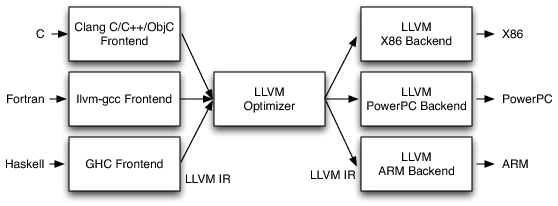
\includegraphics[width=0.8\linewidth]{img/llvm_struct.png}
\end{figure}
\end{frame}

\begin{frame}[fragile]
\frametitle{LLVM - Internal aspects}
\begin{itemize}
  \item Intermediate Representation (IR)
  \begin{itemize}
    \item Mostly architecture-independent instruction set (RISC)
    \item Strongly typed
    \item Unlimited number of virtual registers in SSA
  \end{itemize}
  \item IR Code example:
\end{itemize}

\begin{lstlisting}
      define i32 @main() #0 {
      entry:
        %retval = alloca i32, align 4
        %c = alloca i32, align 4
        store i32 0, i32* %retval, align 4
        %0 = load i32, i32* @a, align 4
        %1 = load i32, i32* @b, align 4
        %add = add nsw i32 %0, %1
        store i32 %add, i32* %c, align 4
        ret i32 0
      }
\end{lstlisting}
\end{frame}


%-------------------------------------------------------
\section{Clang}

\begin{frame}
\frametitle{Clang}
\begin{itemize}
  \item Frontend C/C++, Objective C/C++ and OpenCL C for LLVM
  \item Clear and concise diagnostics (error and warning messages)
  \item Natively a cross-compiler: {\fontfamily{qcr}\selectfont -target <triple>}
  \item Sanitizers
  \item Goals
  \begin{itemize}
    \item Designed to be highly compatible with GCC
    \item C++14 supported since Clang 3.4
    \item C++17 supported since Clang 5
  \end{itemize}
  \item Performance vs GCC ?\footnote{\url{http://www.phoronix.com/vr.php?view=25742}}
\end{itemize}
\end{frame}
%-------------------------------------------------------
\section{Who is using LLVM/Clang}

\begin{frame}
\frametitle{Who is using LLVM/Clang}
\begin{itemize}
  \item Android: Renderscript compiler based on LLVM
  \item Apple
  \begin{itemize}
    \item All operating systems built with LLVM
    \item Xcode IDE uses Clang compiler and static analyzer by default
  \end{itemize}
  \item FreeBSD can be entirely built with Clang/LLVM
  \item Google is using Clang for building:
  \begin{itemize}
    \item Android user space
    \item Chrome on Linux
  \end{itemize}
  \item OpenCL: AMD, Apple, Intel, NVidia (runtime compiler)
  \item Sony Interactive Entretainment: CPU compiler for PS4
\end{itemize}
\end{frame}
%-------------------------------------------------------
\section{Compiling Linux with Clang}

\begin{frame}
\frametitle{Compiling Linux with Clang}
\begin{itemize}
  \item Challenges
  \begin{itemize}
    \item Kernel expects to use some GCC behavior that is not supported by Clang:
    \begin{itemize}
      \item Variable Length Arrays inside structures
      \item Nested functions
      \item Explicit register variables
      \item LLVM assembler cannot be used to build the kernel
    \end{itemize}
  \end{itemize}
  \item LLVMLinux Project: Kernel 4.4 and 4.9 built with Clang for x86\_64 and ARM64
  (patches applied)\footnote{https://lwn.net/Articles/734071/}
  \item Still depends on GNU {\fontfamily{qcr}\selectfont gas} and {\fontfamily{qcr}\selectfont ld}
  \item glibc\footnote{https://sourceware.org/glibc/wiki/GlibcMeetsClang} ?
\end{itemize}
\end{frame}
%-------------------------------------------------------
\section{LLVM/Clang integration to Buildroot}

\begin{frame}
\frametitle{LLVM/Clang integration to Buildroot - What does it enable?}
\begin{itemize}
  \item Gallium llvmpipe driver: software rasterizer that uses LLVM to do runtime code generation
  \begin{itemize}
    \item It is the fastest software rasterizer for Mesa3D
  \end{itemize}
  \item OpenSWR for scientific visualization (AVX, AVX2)
  \item Most OpenCL implementations rely on LLVM
\end{itemize}
\end{frame}

\begin{frame}
\frametitle{LLVM/Clang integration to Buildroot - Considerations}
\begin{itemize}
  \item LLVM/Clang versions
  \begin{itemize}
    \item Current version: 5.0.1 - Upcoming release: 6.0.0 on Feb 21
  \end{itemize}
  \item How to decide which packages are compiled with each compiler (GCC/Clang)?
  \begin{itemize}
    \item i.e. Debian packages: 28203 packages have been rebuild. Among them, 1445 (5.1 \%) failed \footnote{http://clang.debian.net/status.php?version=5.0}
  \end{itemize}
  \item Compile kernel with Clang?
  \item Which OpenCL implementation?
  \begin{itemize}
    \item {\fontfamily{qcr}\selectfont Clover}: part of Mesa. OpenCL 1.1 Supported, missing some OpenCL 1.2 functions
    \item {\fontfamily{qcr}\selectfont pocl}: many CPUs, ASIPs (TCE/TTA), NVIDIA GPUs (via CUDA). Approaching OpenCL 1.2 completeness in 2017
    \item {\fontfamily{qcr}\selectfont Beignet}: intel GPUs. Passed conformance for 1.2 in 2015, nearly complete OpenCL 2.0 in 2017
  \end{itemize}
\end{itemize}
\end{frame}

\begin{frame}
\frametitle{LLVM/Clang integration to Buildroot - Existing work}
\begin{itemize}
  \item Series of patches by Romain Naour (9)\footnote{[Buildroot] [RFC\ 0/9]
  Add llvm/clang + openCL}:
  \begin{itemize}
    \item package/llvm: new host package
    \item package/clang: new host package
    \item package/llvm: enable target variant
    \item package/llvm: RFC: install llvm-config in staging
    \item package/clang: enable target variant
    \item package/llvm: add AMDGPU support
    \item package/mesa3d: enable llvm support
    \item package/libclc: new package
    \item package/mesa3d: enable openCL support
  \end{itemize}
\end{itemize}
\end{frame}

\begin{frame}
\frametitle{Available hardware for testing}
\begin{itemize}
  \item Platform 1 - x86\_64 (HP ProBook)
  \begin{itemize}
    \item Processor: AMD A4-3300M Dual Core @ 1.9 GHz
    \item GPU: AMD Radeon Dual Graphics (HD6480G + HD7450M)
  \end{itemize}
  \item Platform 2 - ARM (Raspberry Pi 2 Model B)
  \begin{itemize}
    \item Processor: ARMv7 Cortex-A7 Quad Core @ 900 MHz
    \item GPU: Broadcom Videocore IV
  \end{itemize}
  \item Platform 3 - ARM/AArch64 (Raspberry Pi 3 Model B)
  \begin{itemize}
    \item Processor: ARMv8 Cortex-A53 Quad Core @ 1.2 GHz
    \item GPU: Broadcom Videocore IV
  \end{itemize}
\end{itemize}
\end{frame}

\begin{frame}
\frametitle{Project planning}
\begin{enumerate}
  \item Provide LLVM support for x86, ARM and AArch64
  \item Provide LLVM support for AMDGPU (R600 to GCN)
  \item Enable LLVM support for Mesa 3D:
    \begin{itemize}
      \item Gallium Drivers: llvmpipe, R600, RadeonSI (not tested)
    \end{itemize}
  \item Provide Clang
  \item Activate OpenCL
  \begin{itemize}
    \item AMD GPUs (Clover)
    \item Broadcom Videocore IV (VC4CL)
  \end{itemize}
\end{enumerate}
\end{frame}

\begin{frame}
\frametitle{LLVM package}
\begin{itemize}
  \item CMake-based project
  \begin{itemize}
    \item Buildroot provides a CMake infrastructure \smiley
  \end{itemize}
  \item Plenty of options
  \item Difficult to be cross-compiled
  \begin{itemize}
    \item At least llvm-tblgen must be compiled for the host first
    \item
  \end{itemize}
\end{itemize}
\end{frame}

\begin{frame}
\frametitle{LLVM package - Directory Layout}
\begin{itemize}
  \item llvm/lib/ Most source files are here
  \begin{itemize}
    \item IR
    \item AsmParser
    \item Bitcode
    \item Transforms
    \item Target
  \end{itemize}
  \item llvm/tools/ Executables built out of the libraries \footnote{https://llvm.org/docs/CommandGuide/index.html}
  \begin{itemize}
    \item llvm-as
    \item \textbf{llvm-config}
    \item lli
    \item llc
    \item opt
  \end{itemize}
  \item llvm/utils/ Utilities for working with LLVM source code
  \begin{itemize}
    \item codegen-diff
    \item llvmgrep
    \item \textbf{TableGen}
  \end{itemize}
\end{itemize}
\end{frame}

%-------------------------------------------------------
\begin{frame}
\Huge{\centerline{Questions?}}
\end{frame}

\end{document}
